\chapter[The Impact of Science Capital on Self-Concept in Science][]{The Impact of Science Capital on Self-Concept in Science: A Study of University Students in New Zealand}

The following work was published in Frontiers in Education on the... Coauthors included Kane Meissel$^1$, Kirsten Locke$^{2,3}$ and Dion R.J. O'Neale$^{2,3}$. 

\footnote{$^{1}$School of Learning, Development, and Professional Practice, Faculty of Education and Social Work, University of Auckland, Auckland, New Zealand \\
$^{2}$School of Critical Studies in Education, Faculty of Education and Social Work, The University of Auckland, Auckland, New Zealand \\
$^{2}$Te P\={u}naha Matatini, University of Auckland, Auckland, New Zealand }

The goal of the current article was to build upon the previous chapter which introduced Bourdieu's sociological theory and how it can be applied to science education. Following feedback from colleagues in the STEM Transformation Institute at Florida International University, I began to question how much information can be gained through administrative data. Administrative data can be explored to understand overall patterns in participation, but how much can it really tell us about the forms of science capital available to students, and how this relates to their internal dispositions? To go deeper, the decision was made to administer a survey, tailored to my research questions, to science students at the university of Auckland.


\begin{abstract}
Understanding factors that contribute to students' self-concept in science is an important task in boosting the number of students studying science and retaining students in science fields. A questionnaire was administered to science students at the University of Auckland in New Zealand (N = 693) to test a theoretical model of science self-concept tied to the work of Pierre Bourdieu. In this model, a student's social capital (i.e., relationships with parents, teachers and peers) and cultural capital (i.e., science related resources) are seen as key determinants of a student's belief that science is a domain in which they can succeed. Results from a Structural Equation Model (SEM) show that, of the factors included in the model, exposure to passionate science teachers during high school was the main predictor of science self-concept for our sample of university science students, while having peers who value science was also found to be important. Interestingly, science-related resources and parents’ value of science were not significant predictors of science self-concept, but the number of university generations in the family did have a positive association.  Students who self-identified as male had higher levels of science self-concept, even after accounting for social and cultural factors in our theoretical model.  Implications of these findings are discussed in the context of the field of science education and Bourdieu's sociological theory.
\end{abstract}


\section{Introduction}
\label{intro}
Much research has been dedicated to understanding who chooses to study science at university, and what factors influence retention and completion of university science degrees. One particular factor that is associated with retention is students' science self-concept. Broadly speaking, self-concept is an individual's perception of their self \citep{shavelson1976self}, while science self-concept relates to a individual's belief regarding their general competency in science \citep{jansen2015students}. Understanding students' science self-concept is important for several reasons. Students who feel that they are good at science are more likely to have better outcomes in science classes \citep{uccar2017role,tighezza2014modeling,chang2008science,peters2013examining}, hold aspirations for further study \citep{mujtaba2018students}, and graduate from university \citep{larson2015predicting}. In turn, graduating from university tends to lead to better life outcomes in general \citep{Oreopoulos_2007}, and greater economic outcomes \citep{norton2016mapping,mahoney2013moving}. Research on factors affecting student's self-concept in science also has important implications for governments, as they seek skilled workers in Science, Technology, Engineering and Mathematics (STEM) to help gain economic prosperity and growth \citep{pricewaterhousecoopers2015smart}. In New Zealand, the education system is not only charged with producing an increase in the number of skilled workers in STEM domains, but also with producing confident learners. This message is made clear in the official high school curriculum \citep{NZC}:

\begin{quote}
   The New Zealand Curriculum is a clear statement of what we deem important in education. It takes as its starting point a vision of our young people as lifelong learners who are confident and creative, connected, and actively involved.
\end{quote} 

A wealth of research has shown that disparities in tertiary science participation exist across the intersection of gender, ethnicity and social class \citep{reynolds2011change,meehan2017explaining}. Students from high Socio-Economic Status (SES) backgrounds are more likely to realise tertiary education goals \citep{reynolds2011change}, whilst interest in science also tends to differ across SES, gender \citep{cheryan2017some}, and ethnicity \citep{Wong2016ScienceStudents}. Previous theorists have used metaphors, such as the \textit{gender filter} \citep{Blickenstaff_2005} and the \textit{smog of bias} \citep{Kost_Smith_2010} that consider the way contextual factors impact on student outcomes. For example, \cite{Kost_Smith_2010} argue that gender disparities can not be attributed to one specific factor, but instead there are a range of factors and small effect sizes that combine to produce inequity. Differing levels of self-concept may be one such factor that contributes to the disparities observed in STEM participation. For example research shows that female students tend to report lower levels of self-concept in mathematics and science \citep{Else-Quest2013}, and gender differences in confidence may persist even when accounting for actual achievement \citep{Ellis_2016}.

A student's self-concept does not exist in a vacuum. It is important to consider the factors that relate to students' self-evaluations of their ability in STEM domains. Why do gender, ethnicity, and social class often share a relationship with students' beliefs regarding their competency in science? The goal of this article is to explore the factors affecting science self-concept further, using a theoretical framework that can answer this question. More specifically, we hope to highlight the way in which students' self-concept in science is rooted in societal structures. To do this, we employ the sociological theory of Pierre Bourdieu \citep{Bourdieu1984}. Recent research has made use of Bourdieu's sociological theory as a framework for understanding the uneven patterns in student interests and pursuits in science \citep{archer2013aspires,Archer_2015,turnbull2019bourdieu}. Bourdieu's theory enables us as researchers to place individuals in the context of their environment, and to understand how social, cultural, and historical factors structure the world in which individuals live, and the internal dispositions they hold. The following section outlines Bourdieu's theory in more detail, with specific reference to \textit{science capital} \citep{Archer_2015}.

\section{Bourdieu and Science Capital}
\label{sciencecapital}
While applications of Bourdieu's sociological theory are wide ranging, it has been increasingly used as a theoretical framework to understand student's experience in science education \citep{Archer2015a}. Bourdieu's sociological framework encourages us to explore how resources are distributed across society, and how external structures in society relate to an individual's internal dispositions.  According to \citet{Bourdieu_1986}, resources, or \textit{capital}, can take various forms; such as economic, cultural, and social. Economic capital refers to an individual's financial resources (e.g. money, investments). Cultural capital refers to an individual's non-financial resources, such as the objects they own (e.g. books, clothing, furniture), or the characteristics they embody (e.g. accent, posture). \citet{Bourdieu_1986} defines social capital as that aspect of our relationships with other individuals that enables us to generate economic and cultural capital. With all forms of capital, the value is determined by the \textit{field} in which it is being used. To give a basic example, owning science books may be of value for someone studying in the field of science, but this is of less value to someone studying opera. Contemporary research has applied Bourdieu's sociology to explore student outcomes in the field of science specifically by using the concept of \textit{science capital} \citep{Archer2015a}. Science capital has been described by \cite{Archer2014} as a:
\begin{quote}
conceptual device for collating various types of economic, social and cultural capital that specifically relate to science --- notably those which have the potential to generate, use, or exchange value for individuals or groups to support and enhance their attainment, engagement and/or participation in science.
\end{quote}
Science capital provides a framework that is relatively simple to interpret and can facilitate our understanding of students' access to resources and the value that they derive from them in science. The following section describes the economic, cultural, and social forms of capital that are important to consider when exploring student's self-concept in science.  We begin by describing the importance of financial assets (economic capital) and non-financial assets (cultural capital) in education. We then describe the importance of shared relationships with others (social capital) which can provide access to resources. We summarise these social relationships in terms of teachers, peers, and family. We finish this section with a discussion of how these resources relate to the way in which students may view themselves in the field of science through Bourdieu's concept of \textit{habitus} and the psychological construct of self-concept. 

\subsection{Economic and Cultural Capital}
Simply put, the concept of economic capital refers to an individuals' financial assets (e.g., money). The benefits of economic capital are well studied and relatively easy to interpret. Previous research has shown that family income and wealth are large predictors of educational success \citep{shapiro2013roots, blanden2004family}. In New Zealand, a 30 year longitudinal study conducted by \citet{gibb2012childhood} found that childhood family income is a strong predictor of educational achievement in later life. As outlined by \cite{Bourdieu_1986}, the value of economic capital comes from its exchange value. For example, students from economically wealthy families are likely able to afford books, laptops, and other aids to study. In paying for these objects, students are exchanging economic capital for non-financial assets. Bourdieu categorizes these non-financial assets under the term cultural capital, and it is through cultural capital that educational advantages are accumulated. Recognising the role of non-financial forms of capital, and with it the social relationships that facilitate access to capital, is complex. In doing so, however, we are able to develop a theoretical model of social class that takes into account factors beyond economic wealth. 

Cultural capital refers to the non-financial resources an individual has at their disposal \citep{Bourdieu_1986}. Cultural capital is a complex concept as it is manifested in the objects that one owns (e.g., books, furniture, clothing), or embodied (e.g., in our posture, accent, bodily physique). In the context of science, cultural capital may take the form of objects that are used, such as chemistry sets, laptops, or books. Students may also boost their cultural capital in science with access to other science-related resources, such as visiting science museums \citep{Dawson2014} or after-school science clubs \citep{mujtaba2018students}. Cultural capital can play an important role in students' progression to university study \citep{aschaffenburg1997cultural}. This is echoed in the field of science education, where research has found that access to science related cultural capital is associated with decisions to study science further in high school \citep{mujtaba2018students}, and at university \citep{Lyons_2006}.

The manner in which students embody their cultural capital may also carry different value in science. Scientists are typically viewed as old, white males \citep{Nosek_2009,Barthelemy_2016} and individuals who differ from this stereotype may face barriers to acceptance in the field \citep{ong2005body}. Research has shown that women tend to be viewed as less competent in science solely in terms of their gender in many different roles, whether it involves a student's application to a lab assistant role \citep{Moss_2012}, or students' evaluation of their science teachers quality \citep{Potvin_2016}. 

\subsection{Social Capital}
While economic and cultural capital are important factors to consider in relation to self-concept, social capital is especially important. Social capital refers to value that is gained through relationships with others. This value can be viewed in terms of the economic and cultural capital that can be mobilised through relationships, but also through the impact of relationships on students internal dispositions \citep{Adler2017}. Having social relationships with individuals who hold valuable forms of capital is highly beneficial. For example, for a student studying at university, having parents who also studied at university may lead to better outcomes. These students are not only more likely to have access to educational resources (objectified cultural capital), but they may also be exposed from an early age to an academic way of life (embodied cultural capital). The following section details three valuable sources of social capital for students studying science: teachers, peers, and family.

\subsubsection{Teachers}
One of the most important forms of social capital for students is the student-teacher relationship. The value of this relationship is derived from several factors. Firstly, the content knowledge that teachers hold is an important form of cultural capital for students \citep{goldhaber2000does,wayne2003teacher,keller2017impact}, as it gives students access to knowledge. Students who have access to teachers with more content knowledge are more able to derive value from their relationship. However, it is also important to consider that content knowledge is transmitted as a function of the quality of the student-teacher relationship. The attitudes and behaviours of teachers can significantly impact on the interest students hold in STEM \citep{keller2017impact} and the way in which students see themselves in science. As outlined by theorists such as \cite{bandura1986explanatory} and \cite{siegle2007increasing}, teachers can boost their student's belief that science is somewhere that they belong by encouraging them and recognising their ability. For example, students who feel recognised as being good at physics are more likely to hold further interest in physics \citep{Hazari2017}. Through a Bourdieusian lens, recognition provides a signal to students that the field is somewhere they belong. Studies of classroom environments have continuously shown that positive teacher-student interactions are a strong source of interest in science \citep{osborne2003attitudes,keller2017impact}. \cite{mujtaba2018students} found that encouragement was an especially important influence in students aspirations to study chemistry. The social capital provided by teachers may be particularly important for students choosing to study in fields where they are members of an underrepresented group, or where their capital is undervalued by those with power in the field.


\subsubsection{Peers}
It is also important to consider the impact of students' social relationships with their peers in science outcomes \citep{osborne2003attitudes}. Adolescence is a time where individuals begin to be increasingly influenced by their peers \citep{douvan1966adolescent}, which can impact on academic engagement and achievement \citep{ryan2000peer} and students may be subjected to group norms that influence the decisions they make about future study \citep{brown1986perceptions}. Following this, it is no surprise that individuals belonging to friendship groups that value science are more likely to have motivations to pursue science further \citep{robnett2013friendship}. Other research shows that students' persistence in STEM domains at university may be influenced by their academic peer groups \citep{Ost_2010}.

\subsubsection{Family}
Finally, students' social capital is bolstered by their relationships within the family. Parents' educational expectations for their children is a key predictor of educational aspirations \citep{wu2015early}. In science, \cite{Lyons_2006} found that parents' attitudes towards educational qualifications and encouragement were important factors relating to students' decisions to study science. Students with highly educated parents are also much more likely to fulfil goals of attaining tertiary qualifications \citep{reynolds2011change}, while students with parents who are employed in STEM occupations are more likely to choose to major in STEM at university \citep{moakler2014college}. These findings point to Bourdieu's concept of social reproduction, where the social position of families are transferred across generations. Parents who are university educated may be more likely to engage in the concerted cultivation of children --- the process of deliberately building cultural capital that is valued by educational institutions \citep{lareau2011unequal}. Parents from higher SES backgrounds may hold higher educational expectations for their children \citep{carolan2015does}, whilst they may also be more involved in their children's education \citep{cheadle2011quantitative}.  Beyond the deliberate cultivation of their children, parents who studied science at university are also more able to use science-related discourse which is an important manifestation of cultural capital \citep{Lyons_2006,bernstein1971class}.\footnote{It is important to note that we do not suggest that the cultural capital espoused by those who are privileged is `better', only that it carries more value in the field of science education. Even though science is commonly perceived as having a `culture of no culture' \citep{traweek2009beamtimes}, the ways of teaching, assessing, and valuing student's capital is predominantly defined by those with power in the field of science --- historically western, male, and wealthy.}  The role of the family goes beyond typical forms of social capital, as the family provides the context in which individuals develop their identity. For this reason, family-related factors can be strongly tied to Bourdieu's concept of habitus.  

\subsection{Habitus}
As previously discussed, students' experiences within fields and their interactions with resources may begin to be embodied physically as embodied cultural capital. At the same time, students also embody these experiences \textit{mentally}. The mental embodiment of capital can be summarised by Bourdieu's concept  of \textit{habitus}. Bourdieu defines habitus as the internal dispositions that an individual holds that generate practices within the field. While an individual's volume of capital may determine their position in the field, their habitus determines their disposition towards the field \citep{bourdieu1992invitation}. Habitus represents an individuals' internalisation of society --- the resulting mental structure of the process commonly referred to as socialisation \citep{Nash1999}.

For Bourdieu, habitus is the mechanism which mediates between structure and agency. Students internalise the environment in which they are placed and make judgements on what is possible and realistic ``for them''. A student's family background is likely to have an integral role in shaping habitus. Students from families that are familiar with university or that have a history of working in science related fields may be more likely to have internalised dispositions that see science as something that is for them. A student's habitus is influenced by their familial context \citep{Dimaggio1982}, with some theorists pointing to the concept of ``family habitus'' as a tool to understand how family resources, values, and lifestyle choices are internalised by children \citep{Archer2012,tomanovic2004family}. The resources available to students through their family are thus extremely important, not only because they offer objectified forms of cultural capital, but also because they offer exposure to ways of thinking and understanding that have been historically proven to be valued by educational institutions. Students may be more likely to view science as a realistic study choice, and university as a possible destination, if they have parents who have modelled these trajectories previously \citep{Lyons_2006}. 

While family provides the context in which habitus is established, habitus is also informed by broader cultural groupings that individual identify with, and their experiences in other contexts, such as school. \citet[p.101]{Bourdieu1984} stated that if individuals are exposed to ``homogenous conditions of existence'' (i.e., similar life experiences) individuals will have similar habitus. In this sense, habitus can take on a collective quality where members of the same group are socialised in similar ways, predisposing them to hold similar dispositions. For example, \citet{Edgerton2014} use the concept of \textit{gendered habitus} to explain how gender socialisation relates to gender disparities in educational achievement. Research also suggests that  contexts outside of the family, such as school and peer groups, become increasingly important as students progress through education, while the impact of the family may diminish \citep{holm2011dealing}.   

Much research has discussed applications of habitus in education research \citep{Reay_2004,Nash1999}, although the concept is often criticised for being too complex \citep{goldhaber2000does} and difficult to operationalise \citep{dumais2002cultural}. Most research on habitus has been qualitative, but, as outlined by \cite{mu2014heritage}, there is an increasing need to consider quantitative applications of habitus. As habitus represents the internalisation of broader social structures, it takes on a collective quality that operates across social groups. While qualitative methods may be more able to describe individual experiences of habitus, quantitative methods are able to explore this collective quality of habitus. The current study  operationalises habitus quantitatively through the use of a science self-concept inventory. The construct of science self-concept was chosen as it is can be theoretically tied to arguments outlined by Bourdieu regarding habitus \citep{mu2014heritage,bodovski2014adolescents}. The following sections will describe self-concept in more detail and explain its relevance to Bourdieu's theory and the current study.   

\subsection{Self-concept}
\label{selfconcept}
While quantitative applications of habitus in education research are relatively rare, quantitative applications of self-concept have been more widely used, operationalised and validated \cite[e.g.][]{marsh2014academic,hattie2014self}.   Despite much variety in definitions of self-concept existing in research \citep{shavelson1976self}, self-concept can be broadly defined as the way in which an individual perceives their self \citep{rosenberg1979conceiving,shavelson1976self}.  As outlined by \citet[p.488]{shavelson1976self} ``Self-concept may be described as: organized, multifaceted, hierarchical, stable, developmental, evaluative, and differentiable.'' In basic terms, self-concept is an individual's judgement about their general competence in a domain \citep{jansen2015students}, which can be general (i.e. ``I am good at school'') and specific (i.e. ``I am good at science at school''). In many ways, self-concept is thus theoretically similar to habitus. Self-concept \citep[p.488]{shavelson1976self} and habitus \citep{Nash1999} are both multifaceted in that they operate across general and specific domains. They are also both relatively stable \citep[p.488]{shavelson1976self} and durable \citep{Bourdieu1984}, although both are subject to change when influenced by environmental sources located outside of the individual, such as the appraisals of others \citep{bong2003academic}. 

Although we identify similarities between self-concept and habitus, it is important to note that we do not consider them to be two different technical terms referring to the same underlying construct (a \textit{jangle fallacy}). While habitus is the internal, deeper ``system of dispositions'' \cite[p.471]{Bourdieu1984} that generates practice, often operating ``below the level of consciousness'' \cite[p.466]{Bourdieu1984}, self-concept is a perception one has of their self (i.e., ``I am good at science'') . While habitus includes domain-specific self-perceptions of competence, it also encompasses an ``estimation of chances'' \citep[p.76]{bourdieu1977outline} that guides future practices and dispositions (i.e., ``is science \textit{for me}?''). Self-concept may be viewed as an aspect of habitus that can be scrutinised through introspection. This point is argued by \citet[p.395]{bodovski2014adolescents}, who suggests that we may view both general and area-specific self-concepts as ``illustrations of different aspects of habitus.'' 

Despite the conceptual differences between habitus and self-concept, we argue that scores on inventories assessing self-concept can be productively interpreted through a Bourdieusian framework, and this has been evidenced in prior research \citep{dumais2002cultural}. As habitus may operate under the surface or unconsciously, it is a difficult concept to measure psychometrically, while self-concept is easier to assess. Importantly, the decision to interpret self-concept in terms of student habitus is necessary as it: ``ensures that the research focus is always broader than the specific focus under study'' \citep{Reay_2004}. In other words, using the concept of habitus facilitates the understanding of how an individual's self-concept is generated in relation to the socio-cultural context in which an individual lives. Given the similarities between self-concept and habitus, self-concept inventories are an appropriate and useful tool to explore an individual's habitus. 

Few New Zealand based studies have explored university students' self-concept or beliefs regarding their academic competency \citep{dalgety2006exploring,murphy2018determinants}. In one such study, \cite{dalgety2006exploring} explored the self-efficacy of first year university chemistry students in New Zealand across three time points in an academic year. They found male students tended to report higher scores in specific items related to self-efficacy (for example in their belief that they could achieve a passing grade in a chemical hazards course). While the work of \cite{dalgety2006exploring} offers many insights into student's internal dispositions at university in the context of New Zealand, the lack of research in this area, especially within the last decade, is a lacuna to be filled. 

\subsection{The Current Study}
\label{sec:3}

The current study seeks to address these two gaps in the research by exploring the relationship between science capital and self-concept in science for university students in New Zealand. More specifically, we apply Pierre Bourdieu's \citep{Bourdieu_1986,Bourdieu1984} concepts of capital and habitus to explore the interaction between students' access to resources and internal dispositions. Whilst the factors affecting outcomes in science are wide-ranging 
\citep{osborne2003attitudes}, we focus on the impact of science-related resources and social experiences in science on students' self-concept in science. In doing so, we are able to assess the impact of social class on self-concept, but using a definition of class defined in terms of \textit{capital} (social, cultural, and economic resources), as opposed to solely economic wealth. Our specific hypotheses are as follows. We expect:
\begin{itemize}
    \item Higher levels of science-related social and cultural capital to be associated with higher levels of self-concept in science. 
    \item Relationships with high school teachers will be the most important form of social capital. This is based on the idea that teachers are experts in the field and their judgements provide the most domain-specific feedback. In terms of habitus, students will be more likely to internalise the idea that they are good at science if they have an expert (the teacher) encourage them and/or recognise their ability. 
    \item Male students will have higher levels of self-concept than female students. This is based on previous research that points to gender disparities in confidence in science and mathematics \citep{Else-Quest2013,Ellis_2016}. 
    \item The number of university generations within a student's family, and having parents positively orientated towards science will be positively associated with self-concept. We would expect students who have available academic role models in their family to have a habitus that is predisposed to university science study. Such students will be more likely to  hold the belief that university is somewhere where they belong, and somewhere that they can be successful, because that is what their family does. 
\end{itemize}
While acknowledging that differences in science self-concept may exist across ethnic groups, the decision was made to exclude ethnicity from the current study. This decision was made to be consistent with kaupapa M\={a}ori values, a research position specific to the context of New Zealand that acknowledges the right of M\={a}ori (the indigenous population of New Zealand) to self-determination. This means that research concerning M\={a}ori should be done with M\={a}ori, and for the benefit of M\={a}ori \citep{walker2006exploration}. We seek to acknowledge our responsibility as researchers by elucidating the patterns found in the current study through a separate qualitative research project. This approach enables students from historically marginalised groups, such as M\={a}ori and Pasifika, the opportunity to have their own voices heard. This qualitative piece seeks to minimise the risk of deficit-theorising by allowing for more depth and nuanced understandings of M\={a}ori and Pasifika experiences in science. Future work should consider ways of knowing and constructing science and culture that are grounded in M\={a}ori ways of knowing, such as M\={a}tauranga \citep{hikuroa2017matauranga}. We hope that the results of the current study can aid in this endeavour.

\section{Methodology}
\label{method}
%\subsection{Data}
%\label{data}
During the first semester of 2019, an online questionnaire was administered to science students at the University of Auckalnd (UoA) via email following approval from the UoA Human Ethics Committee. In order to boost the rate of response, the questionnaire was designed to be quick (10 minutes), consisting of 48 items. Questionnaire responses were anonymous, with the exception of students who left their email to be entered into a prize draw. In total, 693 students consented to participation and completed the questionnaire, with a mean age of around 19 years old (the sample is summarised in Table \ref{tab:Sample}). 

\begin{table}[ht]
\centering

\begin{tabular}{lcccc}
\hline
& N   & Count & Percent    \\ \hline
Male                                                         & 685 & 247 & 0.36   \\
Female                                                       & 685 & 431 & 0.63   \\
Gender Diverse                                               & 685 & 7 & 0.01   \\
Euro                                                         & 693 & 367 & 0.53   \\
Asian                                                        & 693 & 305 & 0.44   \\
Pasifika                                                      & 693 & 28 & 0.04    \\
M\={a}ori                                                        & 693 & 48 & 0.07 \\
MELAA*                                                        & 693 & 21 & 0.03  \\
Other Ethnicity                                               & 693 & \textit{S} & 0   \\
& & &  \\ \hline
& N & Mean & SD \\\hline 
Age** & 594 & 19.93 & 3.65 \\
Parent Job  (0-4) &  681 & 2.61 & 0.71 \\
Uni generations (0-3)                                        & 687 & 1.67 & 1.04 \\ \hline
\end{tabular}
\caption{Sample description. Counts and percentages of categorical characteristics, and means and standard deviations of ordinal characteristics. Individuals self-reported gender which was then categorised into male, female and gender diverse groups for reporting purposes. Participants were given the option to  self-identify with multiple ethnic groups, which means that percentages do not total to 100.  *Middle Eastern, Latin American, or African. **Mature students (those with a recorded age over 24) were excluded from analysis (n $=$ 42). \textit{S} suppressed due to low cell size.} 
\label{tab:Sample}       % Give a unique label
\end{table}

The questionnaire asked students for factual information about themselves, and also questions regarding five latent constructs informed by and adapted from the work of \cite{dewitt2011high}. The constructs, outlined in our conceptual model (see Figure \ref{fig:ConceptualModel_C4}), included self-concept in science (Science Self-Concept; 5 items), experience of high school science teacher quality (Science Teachers; 5 items), parental attitudes towards science (Science Parents; 4 items), peer attitudes towards science (Science Peers; 4 items), and access to science-related resources (Science Resources; 5 items). The first four constructs were measured through items asking students to rate their agreement regarding a statement on a Visual Analog Scale (VAS), with scores ranging from 0 (do not agree) to 100 (strongly agree). VAS have been used extensively in past research and have been found to be as valid and easy to use as likert scales \citep{hasson2005validation}. Given the sample population in the current study can be expected to have high scores on the constructs measured (i.e., in general, we would expect students who choose to study science to score highly on science self-concept measures) there is the possibility of a ceiling effect that could occur with likert scales \citep{chyung2018evidence}. A continuous rating scale was thus used to decrease the risk of a ceiling effect and provide sufficient variance needed for analysis \citep{chyung2018evidence}. The final construct, access to Science Resources, was measured on a 1--5 scale, where students were asked how often they participated in a science related activity (1 being never, 5 being once a week). For all constructs, item statements and loadings can be seen in Table \ref{tab:ItemMeansSDs}. These loadings refer to the extent to which an item relates to the underlying latent construct, and may be interpreted similarly to a correlation (i.e., loadings close to 1 indicate an item strongly loads onto a construct, while loadings closer to 0 are weaker). Other questions asked for factual information, such as gender, ethnicity, family education, and parents' job. 
\begin{figure*}
 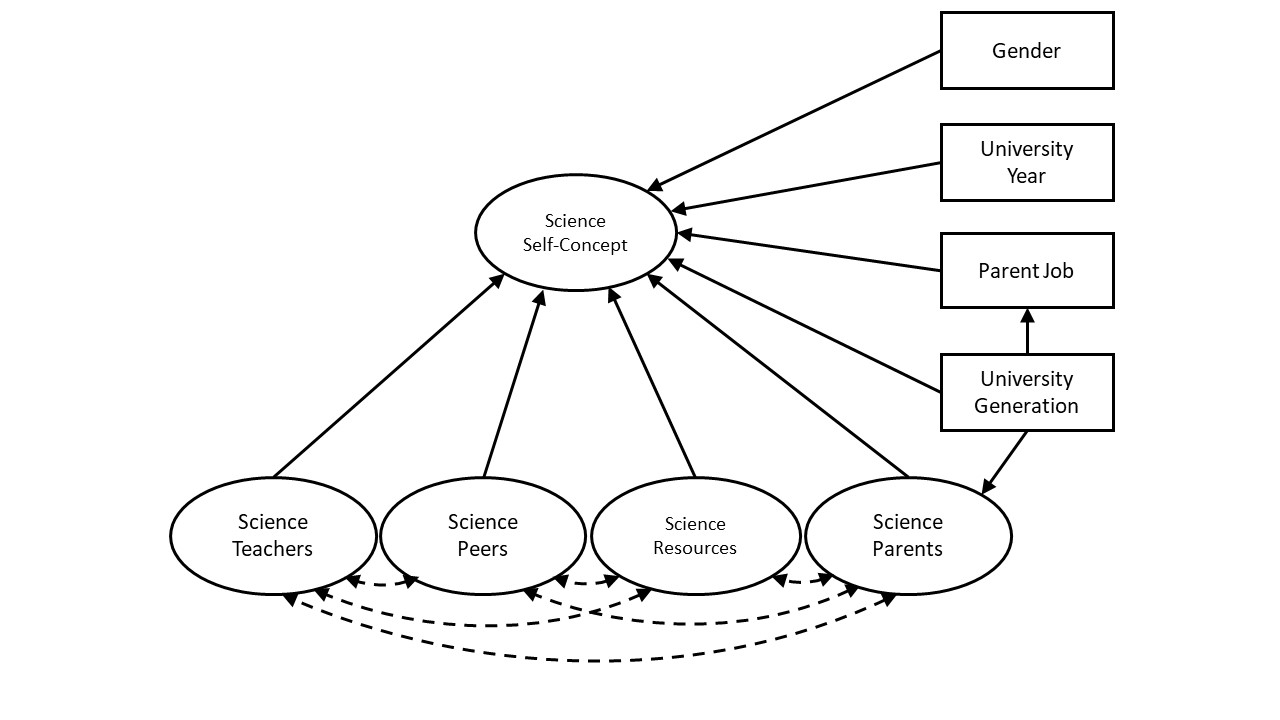
\includegraphics[width = \linewidth]{C4 - Science Capital Self-Concept/ConceptualModel.jpg}
\caption{Conceptual Model. Latent variables are represented by oval boxes, observed variables are represented by rectangular boxes. Regressions are represented by one-sided arrows, while correlations are represented by double headed arrows and dashed lines. }
\label{fig:ConceptualModel_C4}       
\end{figure*}


The following variables were included in our analyses:
\begin{itemize}
    \item \textbf{Science Self-Concept:} We included 5 items from the positive and negative self-concept scales of \cite{dewitt2011high} (``I am good at science'', ``If I study hard I will do well in science courses'').   
    \item \textbf{Science Teachers:} Experience of high school science teachers refers to the extent to which students recall having positive experiences with their high school science teachers. This scale, which included 5 items, refers to the degree of enthusiasm, care and recognition the student perceived. 
    \item \textbf{Science Parents:} Parental attitudes towards science was adapted from the parental attitudes towards science scale of \cite{dewitt2011high} and included 4 items. The item ``My parents would be happy if I became a scientist when I grow up'' was replaced with ``My parents/carers would like it if I worked in science'' to better reflect the target population.
    \item \textbf{Science Peers:} Peer value of science was measured through 4 items adapted from the ``Peer orientation towards school'' and ``Peer attitudes towards science'' scales of \cite{dewitt2011high}. One item, Q4.1 (``My friends see me as a `science' person''), did not load on to the construct. It is likely that this construct represents the participants view of their peers, as opposed to the students' subjective experience of their peers perception of them.
    \item \textbf{Science Resources:} Students' access to resources was adapted from \cite{dewitt2011high} and included 5 items. To suit our target audience, we replace the original phrase ``How often do you do the following things when you are NOT in school...'', with ``Growing up, how often did you...''. One item, Q5.5 (``Growing up, did you go to a lunchtime or after-school science club?'') did not load onto the construct. This may be due to the low number of students who responded positively to this question. An important point to consider is that we, as researchers, are defining science-related cultural capital in our own terms. Whilst the items used in the current study are by definition forms of capital, we acknowledge that other forms of capital exist and hold value in different socio-cultural contexts.
    \item \textbf{University Generations:} University Generations is a count score of the reported number of consecutive generations a participant's family has gone to university. First generation students receive a score of 0,  participants who report having siblings attend receive a score of 1, participants who report having parents attend university receive a score of 2, and those who reported having parents and grandparents attend receive a score of 3.
    \item \textbf{Parent's Job:} Participants were asked to state the profession of their father/male carer and their mother/female carer. The professions were classified according to the Australian and New Zealand Standard Classification of Occupations (ANZSCO), where a score of 0 is unemployed, 1 is low skilled, and 4 is highly skilled. The Parent's Job score is the maximum value of both parents' scores.
    \item \textbf{Gender}. Gender was recorded using an open text box, and then categorised according to the classification set out by Statistics New Zealand. Of the 693 students who completed the survey, only 1\% did not record a gender. 

\end{itemize}

Little's MCAR test showed that data could be considered missing completely at random ($p = .08$), although patterns of missing data showed that there was attrition bias --- questionnaire items tended to have more missing towards the end of the questionnaire. As a robustness check, all models were ran on the imputed and non-imputed datasets. We found that both sets of data had similar model fit, reliability, and relationships between variables. We proceeded to use multiple imputation in order to avoid list-wise deletion of cases with missing data and retain sample size. Missing data for the construct items were imputed using Predictive Mean Matching (PMM) using the MICE package in R \citep{buuren2010mice}, as PMM offers a suitable method for dealing with non-normal data \citep{little1988missing}. Cases that were missing scores on at least half the items from a construct (37 cases) were excluded from analysis (e.g., with a construct with 5 items, cases missing scores on 2 items would be kept, whilst cases missing scores on 3 or more items would be excluded). Mature students (those with a recorded age over 24) were also excluded (42 cases) as the measures of social and cultural capital employed are limited to the transmission of capital from parents and high school to university. A further 31 students were excluded from analysis due to missing data on non-imputable variables, such as parent's job, university generations, or gender. Imputation allowed us to retain 174 cases that would otherwise be excluded with list-wise deletion, leaving a  sample size of 583 students. 

Confirmatory Factor Analysis (CFA) was carried out to test the validity of our latent constructs. Concurrent and convergent validity \citep{campbell1959convergent} of these measures were established through CFA, and found to be at an adequate level. We used Cronbach's $\alpha$ and McDonald's $\omega$ to test internal consistency, with both providing similar reliability scores. McDonald's $\omega$ and Cronbach's $\alpha$ were adequate for all constructs ($\alpha$ ranging from .75 to .85, $\omega$ ranging from .74 to.86), except Science Self-Concept which had an $\alpha$ of 0.68 and an $\omega$ of .67. Whilst 0.70 is usually considered an acceptable level for internal consistency, it has been argued that $\alpha$ below 0.70 are not uncommon for attitudinal scales \citep{field2012discovering}. The lower internal consistency may also be due to the two negatively worded items (Q1.2 and Q1.5) which had lower loadings compared to the other construct items.

\subsection{Structural Equation Modelling}
Structural Equation Modelling (SEM) was used to analyse the conceptual model outlined in Figure \ref{fig:ConceptualModel_C4}. We chose to use SEM for several reasons. Firstly, SEM is able to consider hypothetical constructs that are not directly observable (such as self-concept). In practice, this means that we do not derive new variables from questionnaire items through a mean score or aggregated sum. Instead, SEM uses parameter estimates which consider measurement error and covariances between items. This is especially important when we may not expect our items to load on to a latent construct equally. Secondly, unlike simple regression models, SEM is able to model multiple relationships between variables. Doing so enables us to consider many statistical relationships in a single relative context. Finally, SEM is a widely used technique with established guidelines for judging the quality of models \citep{schreiber2006reporting}, and publicly available software \citep[e.g.][]{rosseel2012lavaan}.

SEM comprises two parts, the measurement model and the structural model. The measurement model shows the loadings of manifest variables onto each latent construct, while the structural model shows the interrelations between the latent constructs and other variables in the conceptual model \citep{schreiber2006reporting}. In our model, Science Self-Concept is viewed as a dependent variable, predicted by Science Teachers, Science Peers, Science Parents, and Science Resources. We also include other manifest variables as predictors, including Gender, University Generations, University Years, and Parent Job. We also model correlations between our latent constructs; in addition, University Generations is modelled as a predictor of Science Parents and Parent Job.

SEM with robust standard errors \citep{huber1967behavior,white1982maximum} was carried out on five imputed datasets using the Lavaan \citep{rosseel2012lavaan} and semTools \citep{jorgensen2018package} packages in R \citep{team2013r}. Rubin's rules \citep{rubin2004multiple} were used to pool point and standard error estimates across our imputed data sets. 

\section{Results}
\label{results}
Descriptive statistics, including means and standard deviations are summarised in Table \ref{tab:ItemMeansSDs}. Correlations between constructs, shown in Table \ref{tab:Correlations}, show that Science Self-Concept was significantly and positively correlated with each form of science capital explored in the current study. Science Self-Concept was most positively associated with Science Teachers ($r = 0.35$, $p<.001$), and most weakly correlated with Science Resources ($r = 0.16$, $p<.001$). We now detail the results of the SEM which explores the relationships between these constructs while including other factors present in the theoretical model (Figure \ref{fig:ConceptualModel_C4}).


\begin{landscape}
\begin{table}[ht]
\centering
\begin{tabular}[width = \textwidth]{clclccccc}
  \hline
 & Item Statement & Loading & Construct & N & Mean & SD & Skewness & Kurtois \\
  \hline
Q1.1 & \parbox[c]{70mm}{I understand everything in my science courses} & 0.62 & Self-Concept & 617 &68.75 & 19.73& -0.94&0.78\\
Q1.2 &   \parbox[c]{70mm}{I find science difficult} & -0.40 &  Self-Concept & 606 & 50.19 & 24.68 & -0.02&-0.78\\
Q1.3 &   \parbox[c]{70mm}{I get good marks in science tests} & 0.72 &  Self-Concept &617 & 67.50&18.06 & -0.42&0.06\\
Q1.4 &  \parbox[c]{70mm}{If I study hard, I will do well in my science courses} & 0.54 &  Self-Concept &620&86.69 &14.85	 &-1.59&3.53\\
Q1.5 &  \parbox[c]{70mm}{I am just not good at science} & -0.38 &  Self-Concept & 605& 20.41& 19.28& 0.85&-0.07\\
  \hline
Q2.1 &  \parbox[c]{70mm}{\begin{spacing}{0.8}My high school teachers recognised that I was good at science\end{spacing}} & 0.75 & Teachers &615&69.08	 &19.10 & -0.80&-0.28\\
Q2.2 &  \parbox[c]{70mm}{My high school teachers cared whether I understood science} & 0.72 &  Teachers &618&70.61 &26.34 & -0.88&0.01\\
Q2.3 &  \parbox[c]{70mm}{My high school teachers explained to me that science is useful for my future} & 0.64 &  Teachers &615&65.24&27.05 &-0.56	&-0.55	\\
Q2.4 &    \parbox[c]{70mm}{My high school science teachers were enthusiastic about science} & 0.64 &  Teachers &619	&75.74&23.70 & -1.06&0.52	\\
Q2.5 &   \parbox[c]{70mm}{My teachers have specifically encouraged me to continue with science after school} & 0.74 & Teachers &593&52.78&32.75 & -0.10&-1.23\\
  \hline
Q3.1 & \parbox[c]{70mm}{My parents/carers think science is interesting} & 0.59 & Parents &618	&70.62&	23.64	 &-0.75	&0.14  \\
Q3.2 & \parbox[c]{70mm}{My parents/carers think it is important for me to learn science} & 0.88 & Parents &619&65.73&26.46	 &-0.48	&-0.54	\\  
Q3.3 & \parbox[c]{70mm}{My parents/carers would like it if I worked in science} & 0.77 & Parents   &612&66.06&27.28 & -0.56&-0.45\\
Q3.4 & \parbox[c]{70mm}{My parents/carers have explained to me that science is useful for my future} & 0.80 & Parents & 592	&53.65	&31.64	& -0.10	&-1.16	\\  
  \hline
Q4.1 & \parbox[c]{70mm}{My friends see me as a ``science person''} & - & - &  602	&70.23&	28.11 &-0.86&-0.14\\
Q4.2 & \parbox[c]{70mm}{My friends think that science is important} & 0.91 & Peers & 615&68.61&	23.47 & -0.65&-0.03 \\
Q4.3 & \parbox[c]{70mm}{My friends think science is cool} & 0.83 & Peers &617&63.38&25.90 & -0.44&-0.48\\ 
Q4.4 & \parbox[c]{70mm}{My friends care about their university grades} & 0.40 & Peers &619&	81.10&	21.21 &-1.56&2.65 \\
  \hline
Q5.1 & \parbox[c]{70mm}{Growing up, did you do science activities (e.g., science kits, nature walks, do experiments)?}  & 0.55 & Resources& 581	&2.40&0.87 & 0.09&-0.68 \\ 
Q5.2 & \parbox[c]{70mm}{Growing up, did you read books or magazines about science?} & 0.69 & Resources &572	&2.42&1.01 & 0.03&-1.11\\
Q5.3 & \parbox[c]{70mm}{Growing up, did you look up things online about science or nature?} & 0.69 & Resources &592&2.97&0.97 &-0.54&-0.79	\\
Q5.4 & \parbox[c]{70mm}{Growing up, did you watch TV programmes about science or nature?} & 0.62 & Resources &599&2.89&0.91 &-0.43&	-0.64\\
Q5.5 & \parbox[c]{70mm}{Growing up, did you go to a lunchtime or after-school science club?} & - &-&579&1.50&0.93 & 1.65&	1.30\\
   \hline
\end{tabular}
\caption{Questionnaire Items. Table showing the questionnaire items used in the current study, with loadings onto the relevant latent construct where applicable. Descriptive statistics for each item are also reported. All items were scored on a continuous scale of 0--100, with the exception of Q5 items, which were scored on a Likert scale of 1-5.} 
\label{tab:ItemMeansSDs}       % Give a unique label
\end{table}
\end{landscape}

\begin{table}[ht]
\begin{tabular}{lccccc}
\cline{2-6}
                  & \parbox{16mm}{\centering Science\\ Self-Concept} & \parbox{13mm}{\centering Science\\ Teachers} &  \parbox{12mm}{\centering Science\\ Parents} & \parbox{12mm}{\centering Science\\ Peers} & \parbox{12mm}{\centering Science\\ Resources} \\ \hline
Science Self-concept  & 1                & -                & -               & -             & -                 \\
Science Teachers  & 0.35            & 1                & -               & -             & -                 \\
Science Parents   & 0.21            & 0.31            & 1               & -             & -                 \\
Science Peers     & 0.26            & 0.30            & 0.49            & 1             & -                 \\
Science Resources & 0.16            & 0.19            & 0.28           & 0.35         & 1                 \\ \hline
\end{tabular}
\caption{\textbf{Correlations between constructs for CFA.}  Variables were standardized to have a mean of 0 and a standard deviation of 1. CFA = confirmatory factor analysis. N = 583; M = 0; SD = 1.}
\label{tab:Correlations}       % Give a unique label
\end{table}


We performed a SEM analysis with robust standard errors to test the conceptual model shown in Figure \ref{fig:ConceptualModel_C4} on a sample of 583 undergraduate science students. While the hypothesized model appears to be a tolerable fit to the data (CFI = .904; TLI = .885;  RMSEA = .053, gamma-hat =  .928), model fit was improved with the inclusion of two modifications. Specifically, we added two additional correlations between items Q2.1 (``My high school teachers recognised that I was good at science'') and Q2.3 (``My high school teachers explained to me that science is useful for my future''), and items Q2.2 (My high school teachers cared whether I understood science) and Q2.4 (My  high  school  science  teachers  were enthusiastic about science). These correlations make sense theoretically, as Q2.1 and Q2.3 may point to possible expectations from teachers, and Q2.2 and Q2.4 may relate more to how personable teachers were. With these modifications, goodness of fit statistics showed acceptable model fit \citep{hu1999cutoff,steiger2007understanding} ($\chi$ = 598.38, df = 258, CFI = 0.93, TLI = 0.91, RMSEA = 0.05, SMSR = 0.05, gamma-hat = 0.95). As shown in Table \ref{tab:MeasurementModel}, the standardized loadings were all significant and acceptable. 

\begin{landscape}
\begin{table}[ht]
\centering
\begin{tabular}{llrrrrr}
  \hline
Latent & Manifest & Estimate & StandardError & z & p & Standardized \\ 
  \hline
Science Self-Concept & Q1.1 & 1.00 &  &  &  & 0.65 \\ 
   & Q1.2 & -0.80 & 0.11 & -6.99 & $<$ .01 & -0.43 \\ 
   & Q1.3 & 1.03 & 0.09 & 11.00 & $<$ .01 & 0.72 \\ 
   & Q1.4 & 0.61 & 0.07 & 8.80 & $<$ .01 & 0.55 \\ 
   & Q1.5 & -0.60 & 0.08 & -7.70 & $<$ .01 & -0.39 \\ 
  Science Teachers & Q2.1 & 1.00 &  &  &  & 0.75 \\ 
   & Q2.2 & 0.94 & 0.06 & 14.65 & $<$ .01 & 0.70 \\ 
   & Q2.3 & 0.97 & 0.08 & 12.80 & $<$ .01 & 0.72 \\ 
   & Q2.4 & 0.75 & 0.07 & 11.03 & $<$ .01 & 0.62 \\ 
   & Q2.5 & 1.18 & 0.08 & 14.51 & $<$ .01 & 0.74 \\ 
  Science Parents & Q3.1 & 1.00 &  &  &  & 0.59 \\ 
   & Q3.2 & 1.65 & 0.12 & 14.05 & $<$ .01 & 0.88 \\ 
   & Q3.3 & 1.51 & 0.13 & 12.06 & $<$ .01 & 0.77 \\ 
   & Q3.4 & 1.81 & 0.14 & 12.82 & $<$ .01 & 0.82 \\ 
  Science Peers & Q4.2 & 1.00 &  &  &  & 0.93 \\ 
   & Q4.3 & 0.99 & 0.06 & 16.26 & $<$ .01 & 0.82 \\ 
   & Q4.4 & 0.39 & 0.05 & 7.82 & $<$ .01 & 0.41 \\ 
  Science Resources & Q5.1 & 1.00 &  &  &  & 0.56 \\ 
   & Q5.2 & 1.43 & 0.11 & 12.69 & $<$ .01 & 0.69 \\ 
   & Q5.3 & 1.40 & 0.15 & 9.18 & $<$ .01 & 0.69 \\ 
   & Q5.4 & 1.16 & 0.13 & 8.84 & $<$ .01 & 0.63 \\ 
   \hline
\end{tabular}
\caption{\textbf{Measurement Model}. The measurement model summarises the loading of items onto theoretical constructs outlined in Figure \ref{fig:ConceptualModel_C4}. The results of the measurement model show that items loadings were significant and acceptable}
\label{tab:MeasurementModel}       % Give a unique label
\end{table}
\end{landscape}

The structural model, shown in Table \ref{tab:StructuralModel} and visualised in Figure \ref{fig:ConceptualModel_results_C4}, shows the interrelationships of the latent variables (specifically the impact of constructs on Science Self-Concept) and the other observed variables in our conceptual model. Results of the structural model show that Science Teachers had the most impact on students' Science Self-Concept with a significant standardised estimate ($\beta$) of 0.33. Of the other science capital related constructs, Science Peers was the only other significant predictor of Science Self-concept ($\beta =$ 0.16). For the other predictors in our model, the number of university generations in the family (Uni Generations) and identifying as male positively predicted Science Self-concept ($\beta =$ 0.12 and $\beta =$ 0.17 respectively). The number of years a student reported being at university (Uni Years) was a significant negative predictor of Science Self-Concept ($\beta =$ -0.10). 

\begin{landscape}
\begin{table}[ht]
\caption{Structural Model} 

\centering
\begin{tabular}{llrrrrr}
  \hline
 Regressions &  & Estimate & Standard Error & z & p & Standardized $\beta$ \\ 
  \hline

  Science Self-concept & Science Teachers & 0.21 & 0.04 & 5.78 & $<$ .01 & 0.33 \\ 
   & Science Parents & -0.02 & 0.06 & -0.42 & .68 & -0.03 \\ 
   & Science Peers & 0.10 & 0.04 & 2.66 & $<$ .01 & 0.16 \\ 
   & Science Resources & -0.04 & 0.18 & -0.22 & .82 & -0.02 \\ 
   & Parent Job & 0.13 & 0.10 & 1.23 & 0.22 & 0.07 \\ 
   & Uni generations & 0.15 & 0.07 & 2.3 & 0.02 & 0.12 \\ 
   & Male & 0.46 & 0.12 & 3.67 & $<$ .01 & 0.17 \\ 
   & Uni Years & -0.13 & 0.06 & -2.28 & 0.02 & -0.10 \\ 
  Science Parents & Uni generations & 0.25 & 0.06 & 4.10 & $<$ .01 & 0.19 \\ 
  Parent Job & Uni generations & 0.21 & 0.03 & 7.14 & $<$ .01 & 0.32 \\ 
  \hline
Covariances &  &  &  &  & &  \\ 
  \hline
  Science Parents & Science Peers & 1.42 & 0.19 & 7.4 & $<$ .01 & 0.48 \\ 
  Science Teachers & Science Parents & 0.96 & 0.16 & 6.02 & $<$ .01 & 0.35 \\ 
  Science Parents & Science Resources & 0.17 & 0.04 & 4.00 & $<$ .01 & 0.25 \\ 
  Science Teachers & Science Peers & 1.35 & 0.23 & 5.90 & $<$ .01 & 0.31 \\ 
  Science Peers & Science Resources & 0.37 & 0.06 & 5.82 & $<$ .01 & 0.35 \\ 
  Science Teachers & Science Resources & 0.19 & 0.06 & 3.40 & $<$ .01 & 0.20 \\ 
   
   \hline
\end{tabular}
\caption{\textbf{Structural Model}. The structural model summarises the inter-relationships between the constructs identified in the measurement model (Table \ref{tab:MeasurementModel}) and the other variables included in the theoretical model (Figure  \ref{fig:ConceptualModel_C4}). The results of the structural model show that while all of the science capital related constructs (Science Teachers, Science Peers, and Science Resources) are positively and significantly correlated, Science Teachers and Science Peers were the only significant predictors of Science Self-Concept. Of the other variables included in the model, the number of university generations in the family (Uni Generations) and being male (Male) positively and significantly predicted Science Self-Concept. The number of years a student had attended university negatively and significantly predicted Science Self-concept. These results are visualised in Figure \ref{fig:ConceptualModel_results_C4} }
\label{tab:StructuralModel}
\end{table}
\end{landscape}

\begin{figure*}
 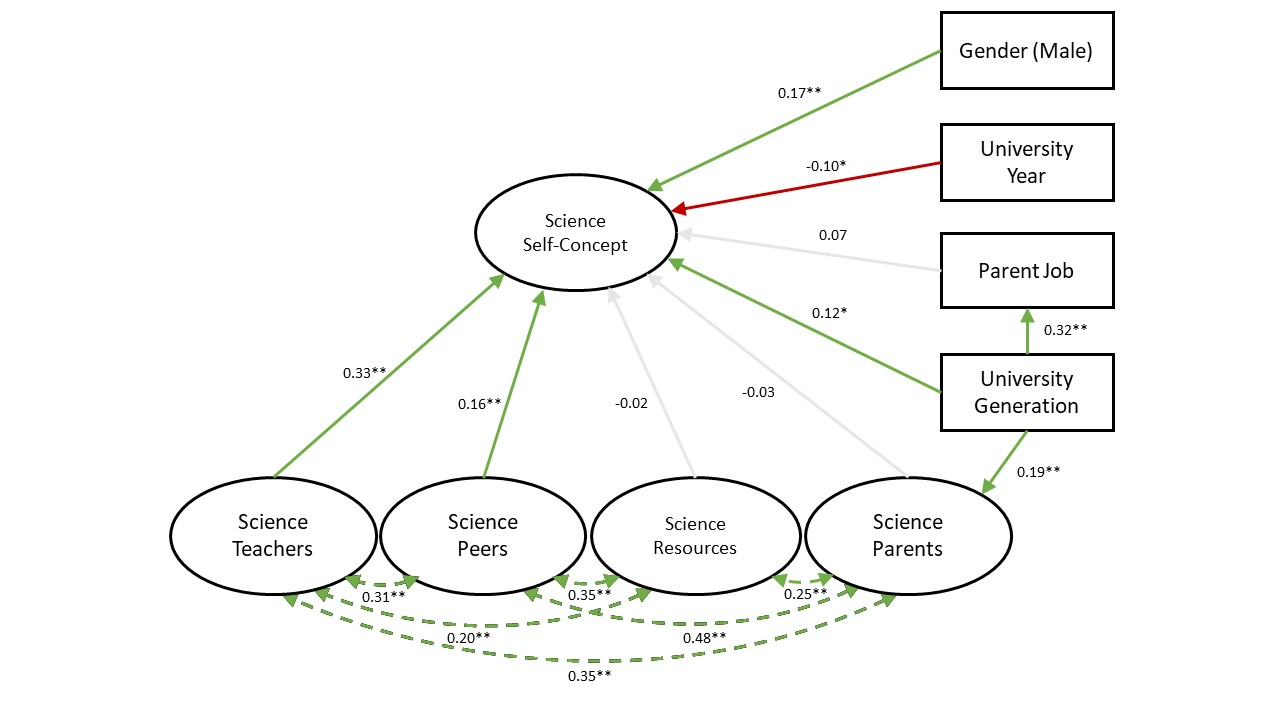
\includegraphics[width = \linewidth]{C4 - Science Capital Self-Concept/ConceptualModel_results.jpg}
\caption{Model results. Results with standardised coefficients and significant of the original conceptual model outlined in Fig \ref{fig:ConceptualModel_C4}. Single headed solid lines indicate a regression, while double headed dotted lines indicate a correlation. Green arrows indicate a positive association, while red indicates a negative association. Faded grey lines indicate no significant relationship. *$p <.05$, **$p <.001$}
\label{fig:ConceptualModel_results_C4}       
\end{figure*}

\section{Discussion}
\label{discussion}
Our results show that, while social capital and cultural capital in science are all positively associated with the science self-concept of university science students, the social relationships shared with teachers and peers are the most important. For university science students, parents' value of science and the science related resources students had while growing up were non-significant predictors of science self-concept. However, the number of university generations within the family did positively predict students' science self-concept. Results also show that male students tended to have higher levels of self-concept, and students who had attended university for more years had lower levels of self-concept. We now discuss these results in the context of university study and New Zealand science education.

Experiences with high school science teachers was the strongest predictor of science self-concept for our sample of university students. While positive experiences were linked to increased science self-concept, negative experiences predicted lower self-concept. Previous research suggests that reflected appraisals from significant others, such as those from teachers, play an important role in the way we view ourselves \citep{bong2003academic}. Tying in with Bourdieu's theory, an individual's habitus is informed by the evidence they see in the field they are participating in. Being recognised as someone who can be successful in science, by a teacher, gives students evidence that they belong. On the other hand, students who have teachers who do not appear to care about them, and who do not encourage them, may internalise the idea that science is not for them. 

The current study was cross-sectional, which means that it may also be the case that students who have low self-concept in science were less likely to have been encouraged by teachers. With that being said, research shows that teachers influence the interests of their students through the support they show students across education levels \citep{marjoribanks2006adolescents}. This process starts as early as primary school \citep{fauth2014student} and through high school \citep{marjoribanks2006adolescents,Hazari2017}. In the field of physics for example, the importance of being recognised as good at physics by teachers has been linked to increased intentions to pursue a career in the field \citep{Hazari2017}. Previous research also shows that students who experience high school teachers who are enthusiastic are more likely to be positively predisposed to the field \citep{keller2017impact}. The current research builds on previous findings by suggesting that positive high school science teachers can positively impact on the self-concept of their students after they leave high school and attend university. Teachers are thus integral to providing safe, inclusive educational environments that are recognised as important for young peoples' well-being \citep{wellbeing2019}. 

Peers' value of science was also positively associated with an individual science self-concept. The mechanism by which friends' value of science has an influence may be linked to social capital. As outlined by \cite{lin1999building}, the value of social capital is not just derived from knowing individuals who can provide access to a broader range of resources and a flow of information. Social capital also helps to build an individual's identity through shared group norms. As suggested by \citet[p.29]{Adler2017}: ``Strong social norms and beliefs\ldots encourage compliance with local rules and customs''. Self-concept may be boosted for students who have more opportunities to talk to others about science in general \citep{Archer2015a}, while receiving increased support from friends \citep{bissell2009role} and/or belonging to a network of friends at university can have positive impacts on persistence \citep{thomas2000ties}. Through a Bourdieusian lens, having a friendship group where students can act out science safely and productively may signal to a student that they belong in science. Students without the same network of support may be less likely to persist in university study \citep{thomas2000ties}. 

It is also likely that individuals with high levels of self-concept in science seek out friends with similar interests. Homophily, the idea that ``birds of a feather flock together'' \citep{mcpherson2001birds}, is a common characteristic of friendship networks. In the case of the current study, students were asked to rate the degree to which their friends think science is important, think science is cool, and care about their university grades. It may be that individuals who responded positively to these items also shared these views previously and formed friendships based on these interests. The social comparisons that students make are also an important source of self-concept \citep{butz2015salient}. Engaging with peers who hold science in high regard and making positive social comparisons to these individuals may be a source of self-concept. Individuals with low levels of self-concept in science may avoid individuals who show great interest in science as social comparisons could make them uncomfortable \citep{bong1999comparison}. The current study is unable to untangle the direction of the relationship between science self-concept and friendship choice, but provides support for future research to investigate this area.   

Parental attitudes regarding science and parental job level were found to have no significant impact on science self-concept. Given research suggests that parent-related factors may impact on adolescent students' academic self-concept \citep{fan2010effects}, we may have expected parents value of science to also positively impact on university students' self-concept in science. However, the impact of family-related variables tends to diminish as students progress through stages of education \citep{holm2011dealing}, and the current study specifically focused on university students which is a late educational stage. It is likely that all three of the family-related factors measured in the current study had a relatively greater impact during earlier stages of a student's educational journey. Whilst parents' value of science likely played a role in the interest that students have in science \citep{archer2013aspires}, parents' values are less likely to play a role in students' science self-concept judgements. The value of social capital is contingent on the context of the task that is being achieved \citep{Adler2017}. As science self-concept is specific to the field of science education, it is reasonable to assume that parents' influence is not as important as teachers and peers who are active actors in the field. Parental attitudes towards science may be more predictive of early interest or engagement in science.  

In contrast to the results for parental attitudes, the number of generations of a student's family that attended university was positively and significantly associated with students' science self-concept. The significance of the number of generations of the student's family who attended university may be related to Bourdieu's concept of cultural reproduction \citep{Dimaggio1982}. The values of parents are transmitted to their children and inform the development of habitus. Students who have university educated parents may be more likely to feel `at home' in a university field. For first generation students, the breaking of new ground may be more confronting and challenging mentally \citep{gardner2011those}. In psychological terms, the internalisation of the idea that ``if my family can do it, so can I'', corresponds to Bandura's \citep{bandura1986explanatory} idea of establishing self-concept through vicarious experience. Seeing someone experience success who is similar to you (i.e., family) may have an especially strong impact on self-concept. With regards to the student's habitus, vicariously experiencing success would help students internalise the idea that university is for \textit{them}. Alternatively, university educated parents may also improve the academic performance of students \citep{paul2011cultural}, which in turn may influence science self-concept. Having family members who attended university is also an important form of social capital, in that it provides students with knowledge on the rules of the field, and what is needed to be successful.

The level of a student's science-related resources growing up, or objectified cultural capital, was found to be non-significant relative to the other factors included in our analysis. It may be that the resources investigated have more importance in generating early interest in science, while students in our sample were already at university. Reading about science and looking things up online about science may relate more strongly to a student's broader interests in science as opposed to their self-concept or self-belief. It may also be that students' social relationships with their teachers and peers (which both positively impacted in self-concept) ameliorate any detrimental effects that a lack of resources would have. The questionnaire items used in this study asked students to recall their access to science-related resources growing up. Future studies should seek to employ a longitudinal research design to more accurately capture the impact of resources on future self-concept in science. 

Students' self-reported gender was significantly related to science self-concept, such that male students, controlling for all other factors, reported higher levels of science self-concept than female students. The lower levels of science self-concept for female students is a common finding in STEM education research \citep{sax2015but,Ellis_2016}. Research has found that students (both male and female) tend to be more likely to make external attributions for a man's failure in science (i.e., the reason for failure is not due to lack of ability, but a poor test or bad luck), but are more likely to attribute women's failure to internal sources (lack of ability) \citep{LaCosse_2016}. 

In a Bourdieusian framework, gender differences in science self-concept can be explained in terms of a `gendered' habitus, a variation of classed habitus \citep{Reay_2004}. This relates to the idea that if individuals are exposed to ``homogenous conditions of existence imposing homogenous conditionings'' individuals will generate ``homogenous systems of dispositions'' \cite[p.101]{Bourdieu1984}. In more basic terms, if individuals are exposed to similar socio-cultural norms and environments, they may be more likely to share similar dispositions. While science has historically been a domain in which men have opportunities to succeed, women face explicit and implicit obstacles \citep{cheryan2017some,Blickenstaff_2005}. These include pervasive negative gender stereotypes \citep{Nosek_2009}, and unfair judgements regarding competency \citep{Moss_2012,Barthelemy_2016}. Men may be more likely to internalise the idea that science is a domain where they belong and can perform, and this may explain why male science students are more likely to hold higher levels of self-concept in science compared to female science students. Although the effect of gender on science self-concept was relatively small, the findings of the current study support the arguments set out by \cite{Kost_Smith_2010} who suggest that the attrition of female students from STEM domains is the result of many small effects that contribute to a ``smog of bias'' where men are bolstered and women face obstacles. 

Finally, the number of years a student reported being at university was found to negatively predict science self-concept. There is a lack of previous research investigating the temporal nature of self-concept in science at university, although one study of a mixed university sample found that academic self-concept may decrease after the first year \citep{isiksal2010comparative}. Other research has found that STEM students' self-efficacy does not decrease from first year to graduation, with it increasing for female students and remaining stable for male students \citep{macphee2013academic}. With regards to the current study, it may be that as students progress through science at university, course content becomes more challenging and thus students may be more likely to report finding science more difficult. Future research should adopt a longitudinal research design to investigate temporal changes in science self-concept in more detail. 

\section{Implications}
The current study provides insights into factors that are related to university students' self-concept in science. The findings reported may inform researchers and policy makers on the cultural and social forms of capital that are required to produce confident learners in science. The current study finds that, for students studying science at university, the social relationships that they have are especially important.

The current study highlights the important role that high school science teachers play in boosting the self-concept of university students. Our results suggest that the impact of high school science teachers continue to be manifested in students' self-concept even after high school is finished and students have entered into university study. Given the importance of self-concept in future achievement \citep{uccar2017role,chang2008science}, the results of the current study suggest that increased teacher support provides a clear method of meeting government aims for increasing the number of skilled workers in science. Massive Open Online Courses (MOOCs) are often cited as a possible solution for teacher shortages, increasing access to education when opportunities are otherwise limited. We argue that even if MOOCs are used, they must still provide students with social connections to teachers who can provide them with real, tangible feedback and recognition. The student-teacher bond should also be the targeted source of intervention to address equity issues in science \citep{banerjee2016systematic}. The expectations that teachers hold for their students may be particularly important \citep{rubie2006teacher}. Research suggests that teacher expectations are an important predictor of students transition to university study, especially for students from low SES backgrounds \citep{gregory2013takes}. 

Our findings also suggest that social relationships with peers who hold science in high regard are linked to science self-concept. This result is especially important to consider for students who originate from social groups that are underrepresented in science and may find it more difficult to form social bonds with other students. Institutional support networks, such as Women in Science, and other community building equity programmes can play an important role in connecting underrepresented students with one another, and help to build a scaffold of peer support \citep{ong2018counterspaces}. Our results also bring attention to the need to ensure that students who are the first generation in their family to attend university are adequately supported in their learning.  

\section{Limitations}
The current study, whilst providing new insights into the factors affecting self-concept of university science students in New Zealand, does have limitations that future studies should seek to address. The questionnaire, short in duration, offered insights into a select group of factors that have been found to be associated with science participation and achievement. The original questionnaire designed by \cite{dewitt2011high} had many other factors that included, but were not limited to, science aspirations, views of scientists, and parental involvement. Furthermore, given the anonymous nature of the questionnaire, it was not possible to link survey responses to administrative data that could give an indication of students' prior or future achievement, and self-reported measures of achievement contained too much missing information to be useful. Prior achievement is likely to account for much of a students' science self-concept and needs to be considered in the context of the current findings.

The sample of students who responded to the survey also display survivorship bias. These are students who have already demonstrated interest and a certain level of success in science. Our study does not account for students who dropped out of science before university. While this may be viewed as a limitation, it also focuses the current study on an \textit{asset-based} framework instead of deficit models of student outcomes. Given our sample of students all demonstrated a certain level of success, we focus on factors that were particularly important for students who made the transition to university science education. Our sample and study design also allows us to identify students who are underrepresented in science based on their demographics or access to capital, but who still recorded high levels of self-concept. A follow-up study will employ a qualitative approach to understand the experiences of these students and refine the directions of future research.

While not reported in our results, our analysis did not find sufficient evidence of measurement invariance across subject disciplines, which suggests that the constructs and relationships outlined in our conceptual model may differ for students by subject. This is not surprising, given the sample sizes per discipline and our generalised measure of science self-concept. Nevertheless, these preliminary results of the SEM suggested that, for our sample, different forms of capital may carry different value across fields, a finding inline with Bourdieu's theory. Each field has its own unique perspective on what forms of capital are valued. While the more general science related factors explored in the current study were found to be associated with a general self-concept in science, specific forms of capital may be particularly important in each science sub-field. For example, mathematics knowledge and self-efficacy in calculus may be more important for students studying in physics \citep{Black2016,Ellis_2016}. More research is needed to identify, summarise, and test the forms of capital that are valued in each science domain. We recommend more in-depth and tailored questionnaires are administered to students per subject discipline.  

\section{Conclusion}
The current study investigated the influence of science-related cultural and social capital (science capital) on the science self-concept of undergraduate science students at the University of Auckland. A Structural Equation Model (SEM) was used to explore the relationships between a set of latent constructs defining science capital and observed measures, such as university generations in the family, parents' employment, and self-identified gender. Our theoretical model provided a good fit to our data, and gives some new insights into the relationship between science capital and science self-concept. We found that, for the students in our sample, positive experiences with high school science teachers was the most important predictor of science self-concept, whilst having peers who value science was also found to be important. Interestingly, we found that reported science-related resources and parents' value of science were not significant predictors of science self-concept, but the number of university generations in the family did have a positive association. These results provide an example of how family culture reproduced over generations may manifest as students' self-belief in the field of university science education. Finally, we also found that students who self-identified as male had higher levels of science self-concept, even after accounting for social and cultural factors in our theoretical model. We discussed these findings in the context of a growing body of research regarding equity in the field of science education, and in the context of Pierre Bourdieu's sociological theory.  

\section{Author Contributions}

SMT, KM, KL, and DO contributed conception and design of the study; SMT administered the questionnaire and organized the database; SMT performed the statistical analysis; SMT wrote the first draft of the manuscript; All authors contributed to manuscript revision, read and approved the submitted version.

%\bibliography{C4 - bib.bib}













